\documentclass[12pt]{article}
\usepackage{amsfonts,amsmath,amssymb,graphicx}
\usepackage[margin=1in]{geometry}

\begin{document}
  \title{Homework 5: \LaTeX}
  \author{Jiashu Han}
  \date{\today}
  \maketitle
  
  \begin{abstract}
  Overall this course is well designed and it is better than all other classes I'm taking this semester, but I think a few things can be changed. These include a slower pace and more explanation of concepts.
  \end{abstract}

  \section{The Good}
  The instructors are enthusiastic and always prepared. Email is a great way to communicate and I always get my questions answered with detailed explanations. Resources are posted online since the beginning of the semester so there's flexibility in the ways of studying.

  \section{The Bad}
  The pace was a little too fast in the middle of the semester when we were covering the FITS files, and I still think I have issues with manipulating the images and FITS files. It would be better if we spend less time working on bash and git and more time on strings and FITS files. 

  \section{The Math}
    \begin{equation}
      \sum_{j=0}^{n} (-1)^{j} \partial^{j}_{\mu_{1} \dotsb \mu_{j}} \left(\frac{\partial \mathcal{L}}{\partial f_{i,\mu_1 \dotsb \mu_j}}\right) = 0
      \label{eq:1}
    \end{equation}
    where $\mu_1 \dotsb \mu_j$ are indices that span the number of variables, that is they go from 1 to n. The summation over the $\mu_1 \dotsb \mu_j$ is implied according to Einstein notation.

  \section{The Tables}
    \begin{center}
      \begin{table}
        \centering
        \begin{tabular}{||l|r||}
          \hline
          Food & IDL Commands \\
          \hline
          Rice & Break!!! \\
          Chocolate & Randomu \\
          Cookies & Findgen \\
          \hline
        \end{tabular}
        \caption{Food is important and so is IDL} \label{table:1}
      \end{table}
    \end{center}
    This is Table \ref{table:1}.

  \section{The Lists}
    \begin{enumerate}
      \item \textit{\textbf{Austin McDowell}}
      \item \textit{\textbf{Will Schultz}}
      \item \textit{\textbf{Joe Zalesky}}
      \label{list:1}
    \end{enumerate}
    \begin{itemize}
      \item 7
      \item 8
      \item 9
      \label{list:2}
    \end{itemize}

  \section{The Figures}
    \begin{figure}[htp]
      \centering
      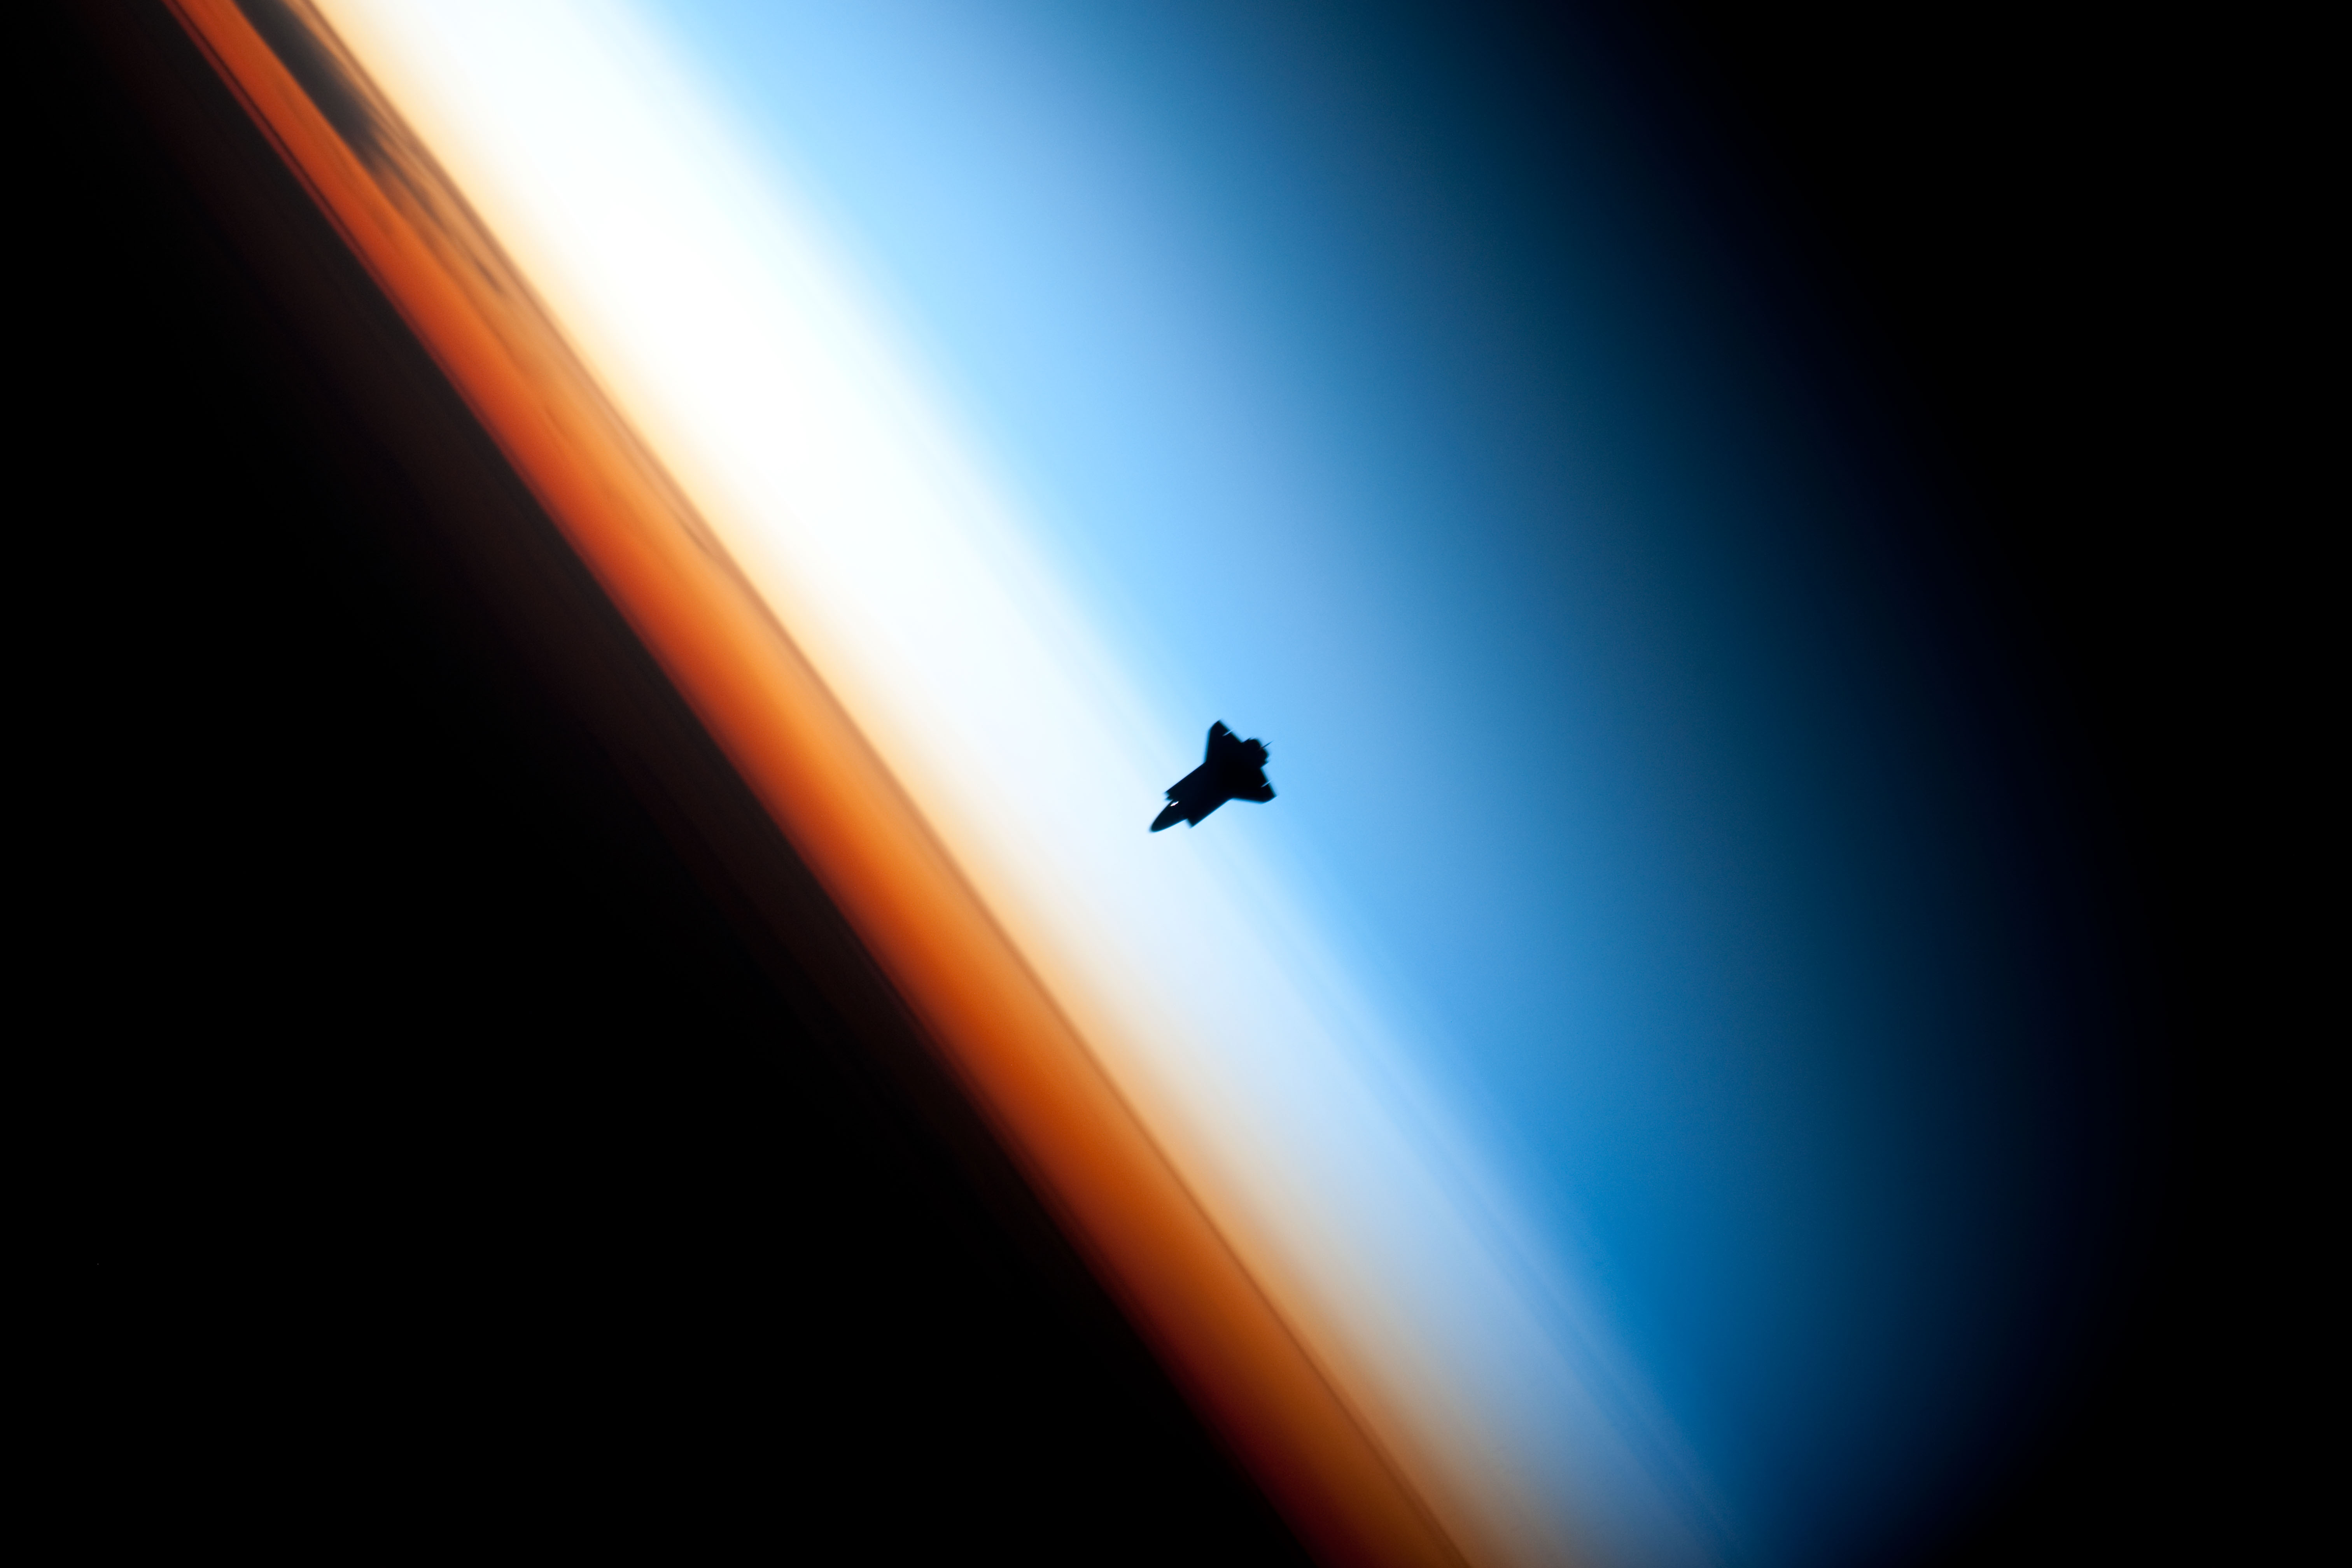
\includegraphics[width=.5\linewidth]{Endeavour_silhouette_STS-130.jpg}
      \label{fig:1}
      \caption{Blue, orange, black, and white are all present. This is my favorite combination. Credit: Expedition 22 crew}
    \end{figure}

  \section{The Comments}
  Life is fabulous!
\end{document}
